\documentclass[xcolor=table]{beamer}

\usepackage{booktabs}
\usepackage{hyperref}
\usepackage[table]{xcolor}
\usepackage{tikz}

\setbeamertemplate{navigation symbols}{}%remove navigation symbols

\title{Next generation consoles and an introduction to normal form games}
\subtitle{Game Theory}
\author{Vincent Knight}
\date{}

\tikzstyle{level 1}=[level distance=3.5cm, sibling distance=3.5cm]
\tikzstyle{level 2}=[level distance=3.5cm, sibling distance=2cm]
\tikzstyle{player} = [text width=4em, draw, text centered, rectangle, fill=blue!20, inner sep=1pt]
\tikzstyle{nature} = [minimum width=3pt,circle,  draw, fill=red!20, inner sep=1pt]
\tikzstyle{end} = [circle, minimum width=3pt, fill, inner sep=0pt, right]

\begin{document}

\frame{\titlepage}


\frame{
\begin{center}
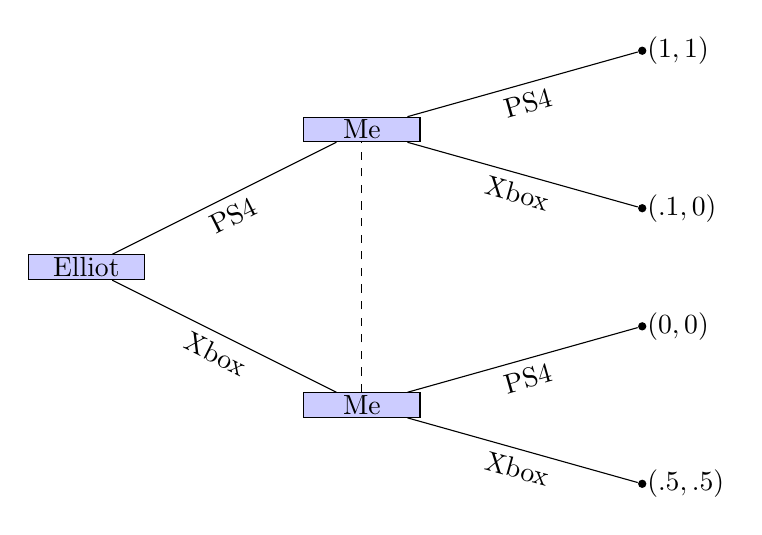
\begin{tikzpicture}[grow=right, sloped]
    \node[player]{Elliot}
        child {node[player] (b) {Me}
                child {node[end] {} node[right] {$(.5,.5)$} edge from parent node[below] {Xbox}}
                child {node[end] {} node[right] {$(0,0)$} edge from parent node[below] {PS4}} edge from parent node[below] {Xbox}}
        child {node[player] (c) {Me}
                child {node[end] {} node[right] {$(.1,0)$} edge from parent node[below] {Xbox}}
                child {node[end] {} node[right] {$(1,1)$} edge from parent node[below] {PS4}} edge from parent node[below] {PS4}};
    \draw[dashed] (b) -- (c);
\end{tikzpicture}
\end{center}
}

\frame{
\begin{itemize}
\item A finite set of $N$ players: Elliot and I.
\item Strategy spaces for the players: $S_1, S_2, S_3, \dots S_N$ - $S_1=S_2=\{\text{Xbox}, \text{PS4}\}$.
\item Payoff functions for the players: $u_i:S_{1}\times S_2\dots\times S_N\to \mathbb{R}$
\end{itemize}
}

\frame{
$$\begin{pmatrix}
(.5,.5)&(.1,0)\\
(0,0)&(1,1)\\
\end{pmatrix}$$
}

\frame{
Mixed strategy: $\sigma_i$
$$\sum_{i=1}^{|S_i|}\sigma_i=1$$
$$\sigma_1=(.3, .7)\text{ and }\sigma_2=(.8,.2)$$
}

\frame{
$$\begin{pmatrix}
(.5,.5)&(.1,0)\\
(0,0)&(1,1)\\
\end{pmatrix}$$

\begin{align*}u_{1}(\sigma_1,\sigma_2)&=\sum_{r\in S_1,s\in S_2}\sigma_1(r)\sigma_2(s)u_{1}(r,s)\\&=.3\times.8\times .5+.3\times.2\times 0+.7\times .8\times .1 + .7\times .2\times 1=.19\\
u_{1}(\sigma_1,\sigma_2)&=\sum_{r\in S_1,s\in S_2}\sigma_1(r)\sigma_2(s)u_{2}(r,s)\\
&=.3\times.8\times .5+.3\times.2\times 0+.7\times .8\times 0 + .7\times .2\times 1=.134
\end{align*}
}

\frame{
\begin{center}
What happens when I `always' buy a PS4?
\end{center}
}

\end{document}
